% Teaser under the title (CVPR-style \twocolumn trick); figure content in figures/method/teaser.png (video/paper_figures)
\twocolumn[{%
\renewcommand\twocolumn[1][]{#1}%
\maketitle
\begin{center}
  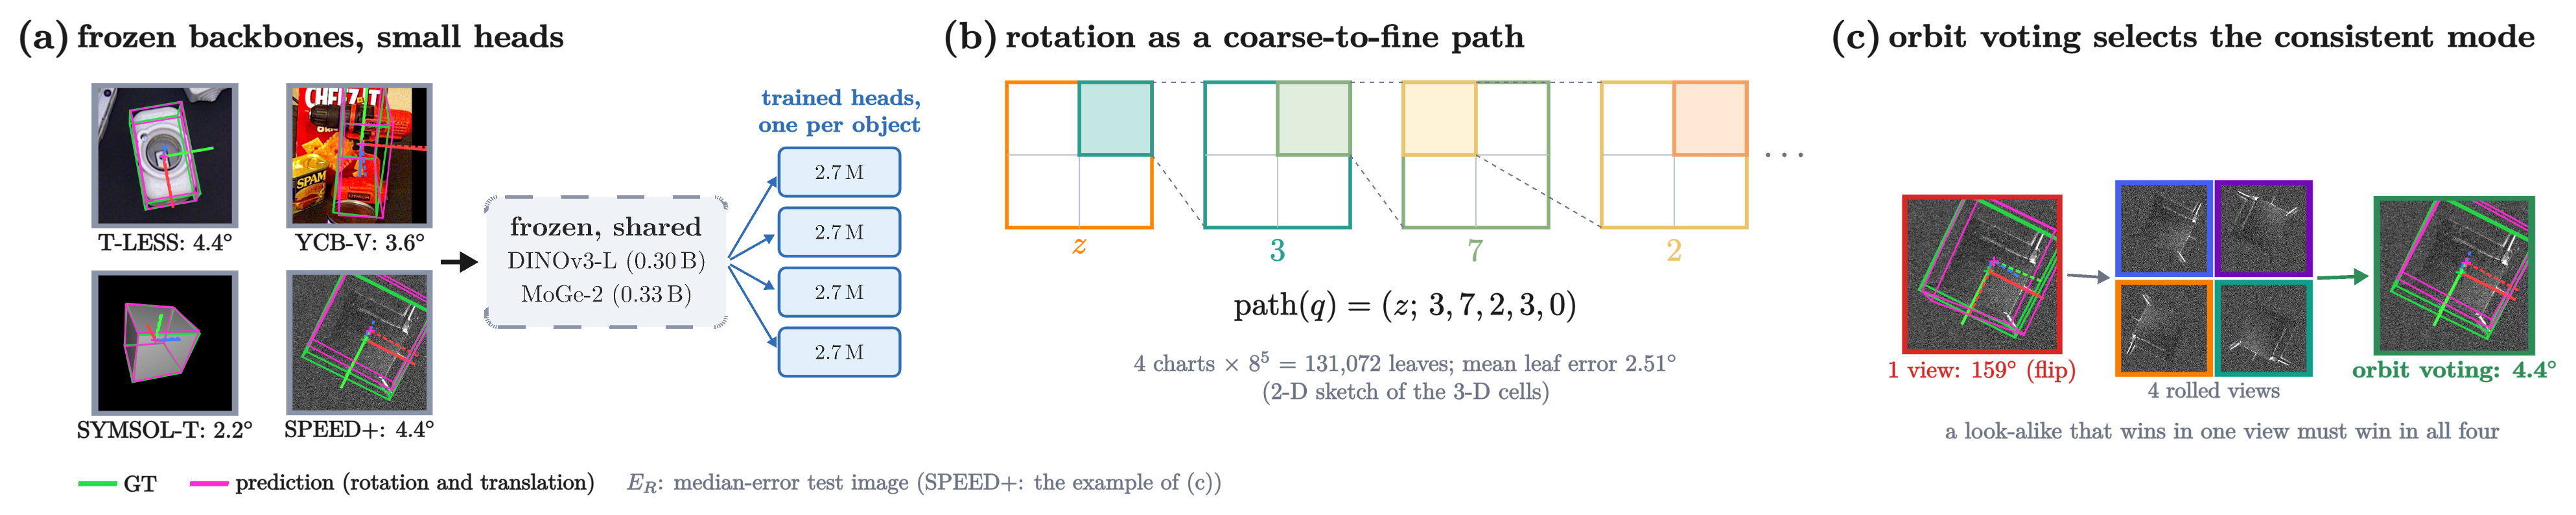
\includegraphics[width=\linewidth]{figures/method/teaser.png}
  \captionof{figure}{\textbf{One frozen design for different known objects.} (a)~Shared, frozen DINOv3 and MoGe-2 backbones feed small heads trained per object (2.7\,M parameters: a 2.4\,M-parameter rotation tree and a 0.33\,M-parameter translation block; the optional MoGe-2 tree adds 2.1\,M); predictions of the final systems on T-LESS, YCB-V, SYMSOL-T and SPEED+ (median-error test image, ground-truth crops; SPEED+ shows the example of (c)). (b)~Rotation is classified as a root-to-leaf path in a hierarchical partition of $SO(3)$ (\cref{fig:tesseract}). (c)~Single-view errors are dominated by look-alike modes, here a $159^\circ$ flip of the near-symmetric spacecraft; orbit voting over four rolled views selects the mode that is consistent in all of them ($4.4^\circ$; \cref{fig:orbit}).}
  \label{fig:teaser}
\end{center}
\vspace{0.5em}
}]
